\documentclass[10pt]{article}         %% What type of document you're writing.
\usepackage{graphicx}
\usepackage{hyperref}
\usepackage[dvipsnames]{xcolor}

%%%%% Preamble

%% Packages to use

\usepackage{amsmath,amsfonts,amssymb}   %% AMS mathematics macros

%% Title Information.

\title{INEGI Data Model}
\author{Adolfo Centeno}
%% \date{2 July 2004}           %% By default, LaTeX uses the current date

%%%%% The Document

\begin{document}

\maketitle

\begin{abstract}
This document implements the INEGI Data Model.
\end{abstract}

\section{Data Model Description}


\textcolor{red}{Entidades} de mexico (\textcolor{green}{ identidad, nombreentidad } ) \\
\textcolor{red}{Municipios}  (\textcolor{green}{ idmunicipio, nombremunicipio} ) \\
\textcolor{red}{Empresas}  (\textcolor{green}{ idempresa, nombreempresa, domicilio, tipoactividad [hospital, escuela, oxxo, gobierno, cajero..], latitud, longitud } ) \\

\begin{enumerate}

\item
Las Entidades se \textcolor{yellow}{componen} de Municipios 
\item
Las Municipios  \textcolor{yellow}{tienen} Empresas 

\end{enumerate}


\section{E-R Model}

INEGI...

\begin{figure}[h]
     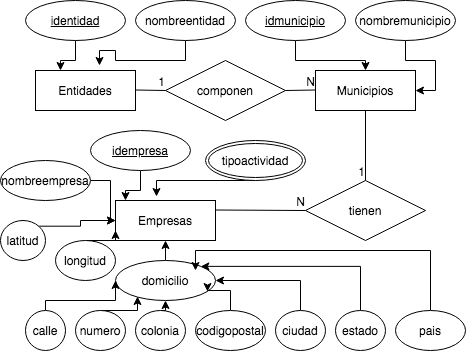
\includegraphics[scale=0.4]{er_inegi}
     \caption{INEGI E-R Model}
\end{figure}
   
\section{Relational Model}
INEGI Relational Model

\begin{figure}[h]
     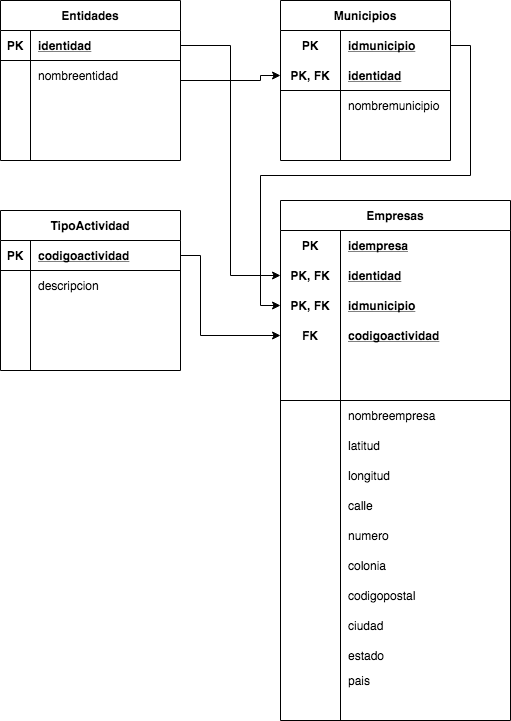
\includegraphics[scale=0.4]{relational_inegi}
     \caption{INEGI Relational Model}
\end{figure}

\end{document}

